Um Softwareprojekte effizient und erfolgreich umzusetzen, ist eine strukturierte Vorgehensweise unerlässlich.
Disziplinorientierte Projektstrukturpläne stellen dabei ein wichtiges Instrument dar, um den Entwicklungsprozess zu planen,
zu steuern und zu überwachen. \\
Das folgende Diagramm zeigt den Projektstrukturplan des Projekts \enquote{flojc. - CarSharing}.
Dieser ist unterteilt in die Disziplinen \enquote{Management}, \enquote{Design}, \enquote{Entwicklung} sowie \enquote{Test und Abnahme}.
Zusätzlich befindet sich eine größere Version des Projektstrukturplans in \autoref{fig:anwendungsfalldiagramm_2}.

\begin{figure}[H]
    \label{fig:anwendungsfalldiagramm}
    \centering
    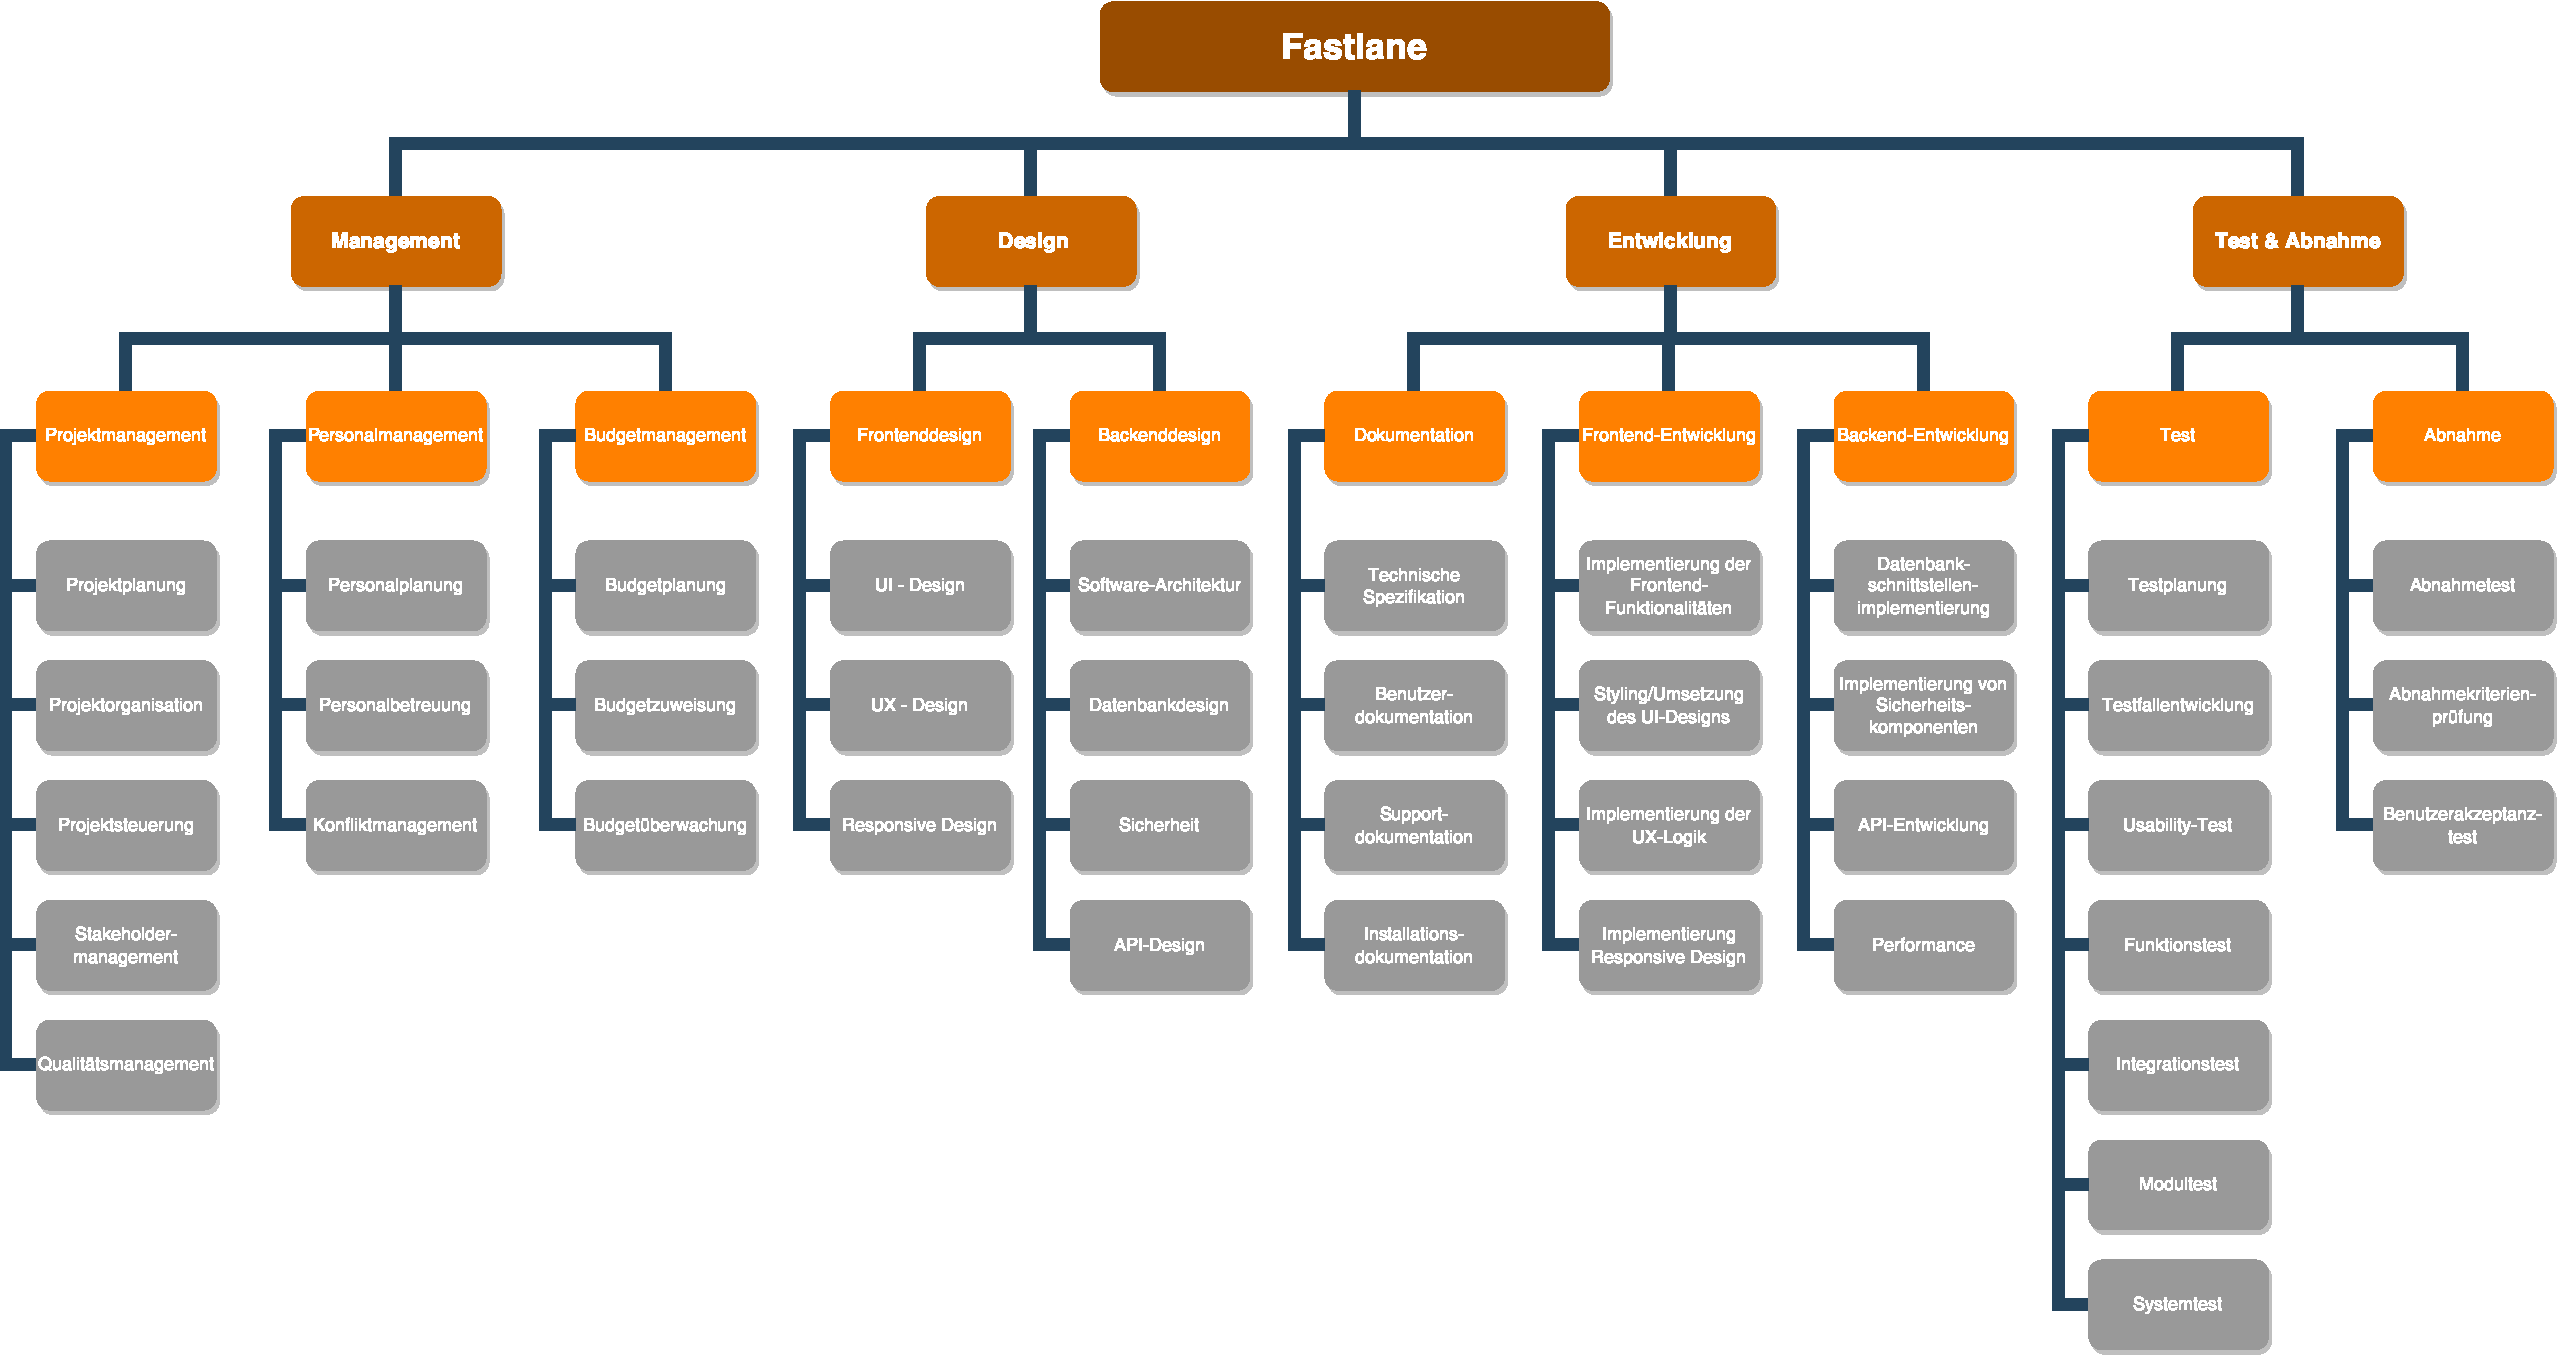
\includegraphics[width = \textwidth]{pictures/Projektstrukturplan}
    \caption{Disziplinorientierter Projektstrukturplan}
\end{figure}